\documentclass[conference]{IEEEtran}
\IEEEoverridecommandlockouts
\usepackage[utf8]{inputenc}
\usepackage[T1]{fontenc}
\usepackage{mathptmx}
\usepackage[spanish,es-noshorthands,es-tabla]{babel}
\usepackage{amsmath,amssymb}
\usepackage{graphicx}
\usepackage{booktabs}
\usepackage{multirow}
\usepackage{array}
\usepackage{xcolor}
\usepackage{tikz}
\usetikzlibrary{positioning,arrows.meta,fit,backgrounds,calc}
\usepackage{cite}
\usepackage[hidelinks]{hyperref}

\newcommand{\TablaCorpus}{LPDP & Perú & 17 & 64 \\
RLPDP & Perú & 60 & 175 \\
RGPD & Unión Europea & 87 & 455 \\
EDPB-07/2020 & Unión Europea & 57 & 237 \\
CCT-2021/915 & Unión Europea & -- & 47 \\}
% Generado por eval/evaluar.py — no editar a mano
\newcommand{\NumFragmentos}{978}
\newcommand{\NumClausulas}{13}
\newcommand{\HitGen}{1{,}000}
\newcommand{\MrrGen}{0{,}772}
\newcommand{\PGen}{0{,}654}
\newcommand{\PeruGen}{0{,}154}
\newcommand{\HitMix}{0{,}923}
\newcommand{\MrrMix}{0{,}733}
\newcommand{\PMix}{0{,}538}
\newcommand{\PeruMix}{0{,}692}
\newcommand{\LatRec}{64}
\newcommand{\Corridas}{3}
\newcommand{\Exactitud}{87{,}2\,\%}
\newcommand{\ExactitudBin}{92{,}3\,\%}
\newcommand{\Estabilidad}{89{,}7\,\%}
\newcommand{\MaePct}{5{,}6}
\newcommand{\LatRev}{32{,}0}
\newcommand{\CitasVer}{98{,}9\,\%}
\newcommand{\TablaContratos}{Completo (NubeSegura) & 100{,}0 & 96{,}8 & 93{,}5--98{,}4 & 89{,}7\,\% \\
Intermedio (PagoFácil) & 59{,}7 & 54{,}8 & 54{,}8--54{,}8 & 92{,}3\,\% \\
Deficiente (MailRápido) & 17{,}7 & 26{,}3 & 21{,}0--30{,}6 & 79{,}5\,\% \\}
\newcommand{\ConfCumpleCumple}{47}
\newcommand{\ConfCumpleParcial}{7}
\newcommand{\ConfCumpleFalta}{0}
\newcommand{\ConfParcialCumple}{2}
\newcommand{\ConfParcialParcial}{18}
\newcommand{\ConfParcialFalta}{1}
\newcommand{\ConfFaltaCumple}{0}
\newcommand{\ConfFaltaParcial}{5}
\newcommand{\ConfFaltaFalta}{37}
\newcommand{\ExactitudVi}{84{,}6\,\%}
\newcommand{\ExactitudBinVi}{87{,}2\,\%}
\newcommand{\EstabilidadVi}{76{,}9\,\%}
\newcommand{\MaePctVi}{8{,}1}
\newcommand{\CitasVerVi}{90{,}8\,\%}


\begin{document}

\title{Agente de Terceros para un Sistema de Gestión de Privacidad Multiagente basado en ISO/IEC 27701:2025: Revisión Asistida de Contratos de Encargo con Recuperación Aumentada}

\author{
\IEEEauthorblockN{Dylan Antonio Zúñiga Huarca, Jeferson Joao Basurco Casani, Adrian Issac Mamani Quispe}
\IEEEauthorblockA{Escuela Profesional de Ingeniería de Sistemas\\
Universidad Nacional de San Agustín de Arequipa, Arequipa, Perú}
}

\maketitle

\begin{abstract}
Cuando una organización encarga a un tercero el tratamiento de datos personales, conserva la responsabilidad sobre esos datos, y el contrato de encargo (DPA) es la principal garantía con la que cuenta. Revisar esos contratos frente a la Ley N.º 29733, su Reglamento (D.S. 016-2024-JUS) y el artículo 28 del RGPD es una tarea manual, repetitiva y propensa a omisiones. Este artículo presenta el \emph{Agente de Terceros}, uno de los ocho agentes de un Sistema de Gestión de Privacidad de la Información (PIMS) multiagente basado en ISO/IEC 27701:2025, responsable de los controles A.1.2.7, A.2.5.7 y A.2.5.8. El agente contrasta cada DPA con \NumClausulas{} cláusulas mínimas mediante recuperación aumentada por generación (RAG): un índice FAISS de \NumFragmentos{} fragmentos normativos con \emph{embeddings} locales (\texttt{nomic-embed-text}) y una única llamada a Gemini 2.5 Flash con salida estructurada. Además, verifica literalmente las citas del modelo, calcula un cumplimiento ponderado, evalúa el riesgo del proveedor con una matriz 4$\times$4, controla vencimientos y subencargados, y somete toda decisión a aprobación humana. Expone sus herramientas por \emph{Model Context Protocol} (MCP) y una interfaz Flask. Una consulta adicional con vocabulario de la norma peruana eleva la cobertura de fuentes peruanas relevantes de \PeruGen{} a \PeruMix{}. Sobre tres contratos anotados y \Corridas{} corridas por contrato, el agente alcanza una exactitud por cláusula de \Exactitud{}, una exactitud binaria (cumple / no cumple) de \ExactitudBin{} y un error absoluto medio de \MaePct{} puntos porcentuales en el índice de cumplimiento.
\end{abstract}

\begin{IEEEkeywords}
Encargado del tratamiento, contrato de encargo, ISO/IEC 27701, gestión de terceros, RAG, sistemas multiagente, Ley 29733, auditoría de sistemas.
\end{IEEEkeywords}

%=====================================================================
\section{Introducción}
Las organizaciones externalizan cada vez más tratamientos de datos personales: alojamiento en la nube, planillas, pasarelas de pago, envío de correos, laboratorios. En todos esos casos el proveedor actúa como \emph{encargado del tratamiento}, y quien le encarga el servicio sigue respondiendo por los datos. La Ley N.º 29733 prohíbe al encargado usar los datos con un fin distinto al del contrato y le obliga a suprimirlos al concluir el servicio (art. 30) \cite{ley29733}. Su Reglamento, aprobado por D.S. N.º 016-2024-JUS, regula la tercerización tecnológica (arts. 28-30), el encargo y la subcontratación (arts. 31-33) y obliga al encargado a informar de inmediato los incidentes de seguridad (art. 36) \cite{ds0162024}. En la Unión Europea, el artículo 28 del RGPD enumera el contenido mínimo del contrato de encargo \cite{rgpd2016}, desarrollado por las Directrices 07/2020 del CEPD \cite{edpb2021} y las cláusulas contractuales tipo de la Decisión (UE) 2021/915 \cite{dec2021915}.

La norma ISO/IEC 27701:2025 convierte el sistema de gestión de privacidad (PIMS) en un estándar independiente y organiza sus controles por rol: la tabla A.1 para responsables, la tabla A.2 para encargados y la tabla A.3 para los controles compartidos \cite{iso27701_2025}. Entre ellos, A.1.2.7 exige contratos con los encargados y A.2.5.7 a A.2.5.9 regulan la divulgación, la contratación y el cambio de subencargados. La gestión de terceros es además un frente de riesgo reconocido en la cadena de suministro \cite{nist800161}.

El equipo de este Trabajo de Investigación Formativa (TIF) diseña un PIMS multiagente con ocho agentes especializados (inventario, riesgos, controles y SoA, evidencias, derechos, incidentes, terceros y formación), coordinados por un orquestador a través de un bus MCP \cite{mcp2025,wang2024agents}. Este artículo describe el \textbf{Agente de Terceros (DPAs)}. Sus contribuciones son:
\begin{itemize}
  \item un catálogo de \NumClausulas{} cláusulas mínimas del contrato de encargo, cada una trazada a la LPDP, al RLPDP, al RGPD y a los controles de ISO/IEC 27701:2025;
  \item un revisor de DPAs basado en RAG con \emph{embeddings} locales y FAISS, que verifica literalmente las citas que produce el modelo;
  \item un modelo de riesgo de proveedores determinista y explicable, más el control de vencimientos, de subencargados y de la aprobación humana (HITL);
  \item una evaluación de la recuperación y de la revisión sobre contratos anotados, con el código y los datos disponibles.
\end{itemize}

%=====================================================================
\section{Marco normativo y trabajos relacionados}

\subsection{El encargado en el Perú y en la Unión Europea}
La Tabla~\ref{tab:comparacion} resume las obligaciones que el agente verifica. La norma peruana es menos detallada que el RGPD sobre el contenido del contrato, pero es más precisa en dos aspectos: fija un plazo máximo de conservación de dos años tras el último encargo (RLPDP art. 31.2) y obliga a evidenciar la supresión (art. 30.4).

\begin{table}[t]
\centering
\caption{Obligaciones del encargado verificadas por el agente}
\label{tab:comparacion}
\footnotesize
\begin{tabular}{@{}p{.27\columnwidth}p{.32\columnwidth}p{.28\columnwidth}@{}}
\toprule
Obligación & Perú (LPDP / RLPDP) & UE (RGPD) \\
\midrule
Fin limitado al contrato & LPDP 30; RLPDP 29.2, 33 & Art. 28.3.a, 28.10 \\
Subencargados & Autorización previa; carga de la prueba del encargado (RLPDP 32) & Autorización previa y aviso de cambios (28.2, 28.4) \\
Seguridad & RLPDP 30.3 & Art. 28.3.c, 32 \\
Incidentes & Informe inmediato (RLPDP 36) & Sin dilación indebida (33.2) \\
Fin del servicio & Supresión evidenciada; hasta 2 años (RLPDP 30.4, 31.2) & Supresión o devolución (28.3.g) \\
Transferencias & LPDP 15; RLPDP 12-14 & Arts. 44-46 \\
\bottomrule
\end{tabular}
\end{table}

\subsection{ISO/IEC 27701:2025}
La edición 2025 reestructura el Anexo A por roles \cite{iso27701_2025}. El texto de la norma no es de libre acceso, así que el agente no lo indexa. En su lugar mantiene un catálogo de los títulos de los controles con una paráfrasis propia. La numeración de 2025 se infiere de la correspondencia con la edición de 2019 \cite{iso27701_2019}: la tabla A.1 corresponde a la cláusula 7 y la tabla A.2 a la cláusula 8, con el último dígito desplazado en uno (por ejemplo, 7.2.6 $\rightarrow$ A.1.2.7 y 8.5.6 $\rightarrow$ A.2.5.7). Esta correspondencia debe confirmarse con el texto oficial.

\subsection{Trabajos relacionados}
La revisión automática de contratos cuenta con conjuntos de datos anotados por expertos como CUAD \cite{hendrycks2021cuad}. Sin embargo, los LLM aplicados al derecho producen afirmaciones no fundamentadas incluso en herramientas comerciales \cite{magesh2024hallucination}. RAG mitiga ese riesgo al condicionar la generación a fragmentos recuperados \cite{lewis2020rag,gao2023survey}. Para la búsqueda vectorial usamos FAISS \cite{johnson2019faiss} y, para los \emph{embeddings}, el modelo abierto \texttt{nomic-embed-text} \cite{nussbaum2024nomic}, que corre en local con Ollama. La aprobación humana sigue el enfoque \emph{human-in-the-loop} \cite{wu2022hitl}, necesario cuando la decisión tiene efectos jurídicos.

%=====================================================================
\section{Arquitectura del agente}
La Fig.~\ref{fig:arq} muestra los componentes. El agente es un paquete de Python con una capa de servicio (\texttt{Agente}) que usan tanto la interfaz web (Flask con HTML, CSS y JavaScript puro) como el servidor MCP. Los datos operativos se guardan en SQLite con un esquema portable a PostgreSQL, que es la base de datos central del PIMS.

\begin{figure}[t]
\centering
\begin{tikzpicture}[font=\scriptsize, node distance=3mm,
  b/.style={draw,rounded corners=2pt,align=center,minimum height=6.5mm,fill=white},
  ext/.style={b,fill=gray!12},
  ar/.style={-Stealth,semithick}]
\node[ext,text width=24mm] (ui) {Interfaz web\\Flask + JS puro};
\node[ext,text width=24mm,right=6mm of ui] (orq) {Orquestador PIMS\\y otros agentes};
\node[b,text width=56mm,below=9mm of $(ui)!.5!(orq)$,fill=blue!6] (ag) {\textbf{Agente de Terceros}\\\texttt{list\_processors} · \texttt{check\_dpa\_status} · \texttt{evaluate\_vendor}};
\node[b,text width=17mm,below left=5mm and -9mm of ag] (rev) {Revisor de DPA\\(13 cláusulas)};
\node[b,text width=15mm,right=2mm of rev] (rie) {Riesgo\\4$\times$4};
\node[b,text width=17mm,right=2mm of rie] (db) {Repositorio\\SQLite + HITL};
\node[b,text width=17mm,below=5mm of rev] (faiss) {FAISS\\\NumFragmentos{} fragm.};
\node[ext,text width=17mm,left=3mm of faiss] (oll) {Ollama\\nomic-embed};
\node[ext,text width=15mm,right=3mm of faiss] (gem) {Gemini 2.5\\Flash (JSON)};
\draw[ar] (ui.south) -- node[fill=white,inner sep=1pt,font=\tiny]{REST} (ui.south |- ag.north);
\draw[ar] (orq.south) -- node[fill=white,inner sep=1pt,font=\tiny]{MCP} (orq.south |- ag.north);
\draw[ar] (ag) -- (rev); \draw[ar] (ag) -- (rie); \draw[ar] (ag) -- (db);
\draw[ar] (rev) -- (faiss); \draw[ar] (oll) -- (faiss); \draw[ar] (rev) -- (gem);
\end{tikzpicture}
\caption{Arquitectura del Agente de Terceros dentro del PIMS multiagente.}
\label{fig:arq}
\end{figure}

Las herramientas expuestas al bus MCP son las definidas para este agente en el diseño del PIMS:
\begin{itemize}
  \item \texttt{list\_processors}: lista los encargados con el estado de su DPA y su nivel de riesgo;
  \item \texttt{check\_dpa\_status}: indica si el DPA está vigente, por vencer (60 días), vencido, pendiente de aprobación o ausente;
  \item \texttt{evaluate\_vendor}: devuelve la evaluación de riesgo con sus factores y recomendaciones;
  \item \texttt{processors\_in\_breach}: apoya al Agente de Incidentes, que ante una brecha necesita saber qué encargados tratan la categoría de datos o el sistema afectado y si su contrato les obliga a notificar.
\end{itemize}

\textbf{Puerta HITL.} Todo DPA revisado y todo cambio de subencargado quedan \emph{pendientes} hasta que Asesoría Legal o el DPO los aprueben o rechacen. Cada acción del agente y cada decisión humana se registra en una bitácora de auditoría (actor, acción, detalle y fecha), que sirve como evidencia para la cláusula 9 de la norma.

%=====================================================================
\section{Metodología}

\subsection{Corpus e indexación}
El corpus (Tabla~\ref{tab:corpus}) combina las normas peruanas, el RGPD y dos fuentes públicas especializadas en el encargo. El texto se extrae con \texttt{pypdf}, se limpia y se fragmenta en párrafos empaquetados hasta 1000 caracteres, con un solape de 150. Cada fragmento conserva su fuente, su jurisdicción, su página y el artículo o la cláusula detectados con expresiones regulares. Los vectores (768 dimensiones, con los prefijos de tarea de \texttt{nomic-embed-text}) se normalizan y se indexan en un \texttt{IndexFlatIP} de FAISS, que equivale a una búsqueda exacta por similitud coseno.

\begin{table}[t]
\centering
\caption{Corpus normativo del agente}
\label{tab:corpus}
\footnotesize
\begin{tabular}{@{}llrr@{}}
\toprule
Sigla & Jurisdicción & Págs. & Fragm. \\
\midrule
\TablaCorpus
\midrule
Total & & & \NumFragmentos \\
\bottomrule
\end{tabular}
\\[2pt]{\scriptsize CCT-2021/915 se obtuvo como texto HTML de EUR-Lex, sin paginación.}
\end{table}

\subsection{Cláusulas mínimas}
La Tabla~\ref{tab:clausulas} lista las \NumClausulas{} cláusulas. Cada una tiene un criterio de cumplimiento, su base normativa, los controles ISO que la sustentan, un peso $w\in\{1,2,3\}$ (recomendable, importante o esencial) y dos consultas de recuperación: una general y otra con el vocabulario de la LPDP y el RLPDP (por ejemplo, ``titular del banco de datos'' o ``subcontratación'').

\begin{table}[t]
\centering
\caption{Cláusulas mínimas del contrato de encargo}
\label{tab:clausulas}
\scriptsize
\begin{tabular}{@{}p{.36\columnwidth}p{.22\columnwidth}p{.24\columnwidth}c@{}}
\toprule
Cláusula & RGPD & ISO 27701 & $w$ \\
\midrule
Objeto, duración, finalidad & 28.3 & A.1.2.7, A.2.2.3 & 3 \\
Instrucciones documentadas & 28.3.a, 29 & A.2.2.3, A.2.2.5 & 3 \\
Confidencialidad & 28.3.b & A.2.2.2 & 2 \\
Medidas de seguridad & 28.3.c, 32 & A.2.2.2, A.2.4.4 & 3 \\
Subencargados & 28.2, 28.4 & A.2.5.7--A.2.5.9 & 3 \\
Derechos de los titulares & 28.3.e & A.2.3.2 & 2 \\
Notificación de incidentes & 28.3.f, 33.2 & A.2.2.2, A.2.2.6 & 3 \\
Supresión o devolución & 28.3.g & A.2.4.3 & 3 \\
Auditorías & 28.3.h & A.2.2.6, A.2.2.7 & 2 \\
Transferencias internacionales & 44--46 & A.2.5.2, A.2.5.3 & 2 \\
Prohibición de fines propios & 28.10 & A.2.2.3 & 3 \\
Solicitudes de autoridades & 28.3.a & A.2.5.5 & 1 \\
Asistencia en EIPD & 28.3.f, 35 & A.2.2.2 & 1 \\
\bottomrule
\end{tabular}
\end{table}

\subsection{Revisión de un DPA}
\begin{enumerate}
  \item \textbf{Recuperación por cláusula.} Para cada cláusula se recuperan seis fragmentos con la consulta general y dos fragmentos peruanos con la consulta local. Los resultados se unen sin duplicados y se ordenan por similitud. La numeración de los fragmentos es global y se comparte entre las cláusulas.
  \item \textbf{Generación.} Una sola llamada a Gemini 2.5 Flash \cite{gemini25} recibe las cláusulas, los fragmentos numerados y el texto del contrato (o, si este supera 30\,000 caracteres, sus fragmentos más pertinentes). Devuelve un JSON con el estado, la cita literal, los fundamentos y la recomendación de cada cláusula. Una sola llamada reduce la latencia y el consumo frente a trece llamadas separadas.
  \item \textbf{Validación.} Se descartan los identificadores desconocidos y los estados inválidos. Una cláusula que el modelo no evalúa cuenta como ``falta''.
  \item \textbf{Verificación literal.} La cita se divide en frases (separadas por punto o por elipsis) y cada frase de 20 caracteres o más debe aparecer en el contrato normalizado. Si una cláusula marcada como ``cumple'' no supera esta verificación, baja a ``parcial'' y se señala para revisión manual.
  \item \textbf{Puntaje.} Con $v(\text{cumple})=1$, $v(\text{parcial})=0{,}5$ y $v(\text{falta})=0$,
  \begin{equation}
    C = 100\,\frac{\sum_i w_i\, v(e_i)}{\sum_i w_i}.
  \end{equation}
\end{enumerate}

\subsection{Riesgo del proveedor}
Siguiendo la gestión del riesgo de la AEPD y la NTP-ISO 31000 \cite{aepd2021,ntp31000}, el riesgo es $R = P \times I$ con $P, I \in \{1,\dots,4\}$. El impacto parte del volumen de titulares (bajo, medio o alto) y suma 1 si se tratan datos sensibles. La probabilidad parte de 1 y suma 1 por cada uno de estos factores: transferencia a un país sin nivel adecuado, uso de subencargados, DPA sin revisar o con $C<70$ y ausencia de un DPA vigente. Los incidentes de los últimos doce meses suman 1, o 2 si son tres o más. La certificación ISO/IEC 27701 resta 1. El nivel es bajo si $R\le3$, medio si $R\le6$, alto si $R\le9$ y crítico en otro caso, con revisiones cada 24, 12, 6 y 3 meses respectivamente. Que el modelo sea determinista es deliberado: el auditor debe poder reproducir el puntaje.

%=====================================================================
\section{Evaluación}

\subsection{Recuperación normativa}
Para cada una de las \NumClausulas{} cláusulas anotamos el conjunto de pares (fuente, artículo) relevantes. En el caso de las Directrices 07/2020, que no tienen artículos, contamos como relevantes las páginas 34 a 48, que desarrollan el contrato de encargo. Medimos Hit@6, MRR y P@6, y además la \emph{cobertura peruana}: la proporción de cláusulas que recuperan al menos un fragmento peruano relevante. Esta métrica importa porque la LPDP y el RLPDP son la norma aplicable al caso.

\begin{table}[t]
\centering
\caption{Recuperación por cláusula (k = 6)}
\label{tab:recuperacion}
\footnotesize
\begin{tabular}{@{}lcccc@{}}
\toprule
Estrategia & Hit@6 & MRR & P@6 & Cob. Perú \\
\midrule
Solo consulta general & \HitGen & \MrrGen & \PGen & \PeruGen \\
General + consulta peruana & \HitMix & \MrrMix & \PMix & \PeruMix \\
\bottomrule
\end{tabular}
\end{table}

La Tabla~\ref{tab:recuperacion} muestra que la búsqueda general recupera casi solo fuentes europeas, mucho más extensas y redactadas con el vocabulario del RGPD. La consulta con vocabulario peruano corrige ese sesgo: la cobertura peruana pasa de \PeruGen{} a \PeruMix{}. El costo es una ligera caída de Hit@6 (de \HitGen{} a \HitMix{}), porque en la cláusula de solicitudes de autoridades los dos fragmentos peruanos empujan fuera de los seis primeros puestos a los dos fragmentos relevantes (RGPD art. 28 y CEPD). En la práctica, el agente envía al modelo la unión completa (hasta ocho fragmentos), no solo los seis primeros. La primera versión del agente colocaba los fragmentos peruanos al inicio de la lista sin importar su similitud: con ella, el MRR caía a 0{,}455 y la cobertura peruana solo llegaba a 0{,}308. Ordenar la unión por similitud y usar una consulta específica para la norma peruana resolvió ambos problemas. La latencia media de recuperación es de \LatRec{}~ms por cláusula, que se reparte entre el \emph{embedding} local de la consulta y la búsqueda en FAISS.

\subsection{Revisión de contratos}
Construimos tres contratos ficticios con distinto grado de cumplimiento: uno completo, que contempla las trece cláusulas; uno intermedio, de una pasarela de pagos con varias cláusulas parciales o ausentes; y uno deficiente, de un servicio de \emph{mailing} que permite usos propios y subencargados sin aviso. Los autores anotaron el estado esperado de cada cláusula ($3\times13=39$ etiquetas). Cada contrato se revisó \Corridas{} veces para medir la variabilidad del LLM.

\begin{table}[t]
\centering
\caption{Índice de cumplimiento $C$ (\%) frente a la referencia}
\label{tab:contratos}
\footnotesize
\begin{tabular}{@{}lcccc@{}}
\toprule
Contrato & Ref. & Media & Rango & Exactitud \\
\midrule
\TablaContratos
\bottomrule
\end{tabular}
\end{table}

\begin{table}[t]
\centering
\caption{Matriz de confusión agregada (filas: referencia; columnas: agente)}
\label{tab:confusion}
\footnotesize
\begin{tabular}{@{}lccc@{}}
\toprule
 & cumple & parcial & falta \\
\midrule
cumple & \ConfCumpleCumple & \ConfCumpleParcial & \ConfCumpleFalta \\
parcial & \ConfParcialCumple & \ConfParcialParcial & \ConfParcialFalta \\
falta & \ConfFaltaCumple & \ConfFaltaParcial & \ConfFaltaFalta \\
\bottomrule
\end{tabular}
\end{table}

El agente obtiene una exactitud por cláusula de \Exactitud{} y una exactitud binaria (cumple frente a no cumple) de \ExactitudBin{}. El error absoluto medio del índice es de \MaePct{} puntos porcentuales (Tabla~\ref{tab:contratos}). El \Estabilidad{} de las cláusulas recibe el mismo estado en las \Corridas{} corridas, y el \CitasVer{} de las citas aportadas supera la verificación literal. La latencia media de una revisión completa es de \LatRev{}~s. La Tabla~\ref{tab:confusion} muestra que todos los errores ocurren entre estados adyacentes: el agente nunca confunde ``cumple'' con ``falta''. Los errores son ambigüedades de grado, el mismo tipo de caso en que dos auditores humanos suelen discrepar. El sesgo depende del contrato. En el completo, el agente es conservador (algunas cláusulas que cumplen quedan como parciales). En el deficiente es algo indulgente: califica como parciales cláusulas ausentes en las que el contrato dice algo relacionado, como la ley aplicable de Delaware en lugar de una cláusula de transferencias. Por eso sobreestima el índice (26{,}3 frente a 17{,}7).

\textbf{Iteración del prompt.} En la primera versión, el prompt pedía ``copiar la frase literal'', pero el modelo a veces resumía o parafraseaba la cita. La verificación literal rechazaba entonces esas citas y degradaba cláusulas que sí se cumplían: en una corrida, 7 de las 13 citas del contrato completo no superaron la verificación y el índice cayó a 67{,}7\,\%. Por eso reforzamos la regla: copiar carácter por carácter una o más frases completas, sin resumir, separando con ``…'' los tramos que estén en lugares distintos. La Tabla~\ref{tab:iteracion} compara ambas versiones sobre los mismos contratos. La verificación literal cumplió su función: impidió que paráfrasis no comprobables contaran como evidencia.

\begin{table}[t]
\centering
\caption{Efecto de la regla de cita literal en el prompt}
\label{tab:iteracion}
\footnotesize
\begin{tabular}{@{}lcc@{}}
\toprule
Métrica & v1 & v2 (final) \\
\midrule
Exactitud por cláusula & \ExactitudVi & \Exactitud \\
Exactitud cumple / no cumple & \ExactitudBinVi & \ExactitudBin \\
Estabilidad entre corridas & \EstabilidadVi & \Estabilidad \\
Error absoluto medio de $C$ (pp) & \MaePctVi & \MaePct \\
Citas que superan la verificación & \CitasVerVi & \CitasVer \\
\bottomrule
\end{tabular}
\end{table}

\subsection{Demostración}
La Fig.~\ref{fig:ui} muestra la ficha de un proveedor de riesgo crítico y el informe de revisión de su contrato. Cada cláusula incluye su estado, la cita del contrato, la recomendación y los fragmentos normativos que la fundamentan, con fuente, artículo y página.

\begin{figure}[t]
\centering
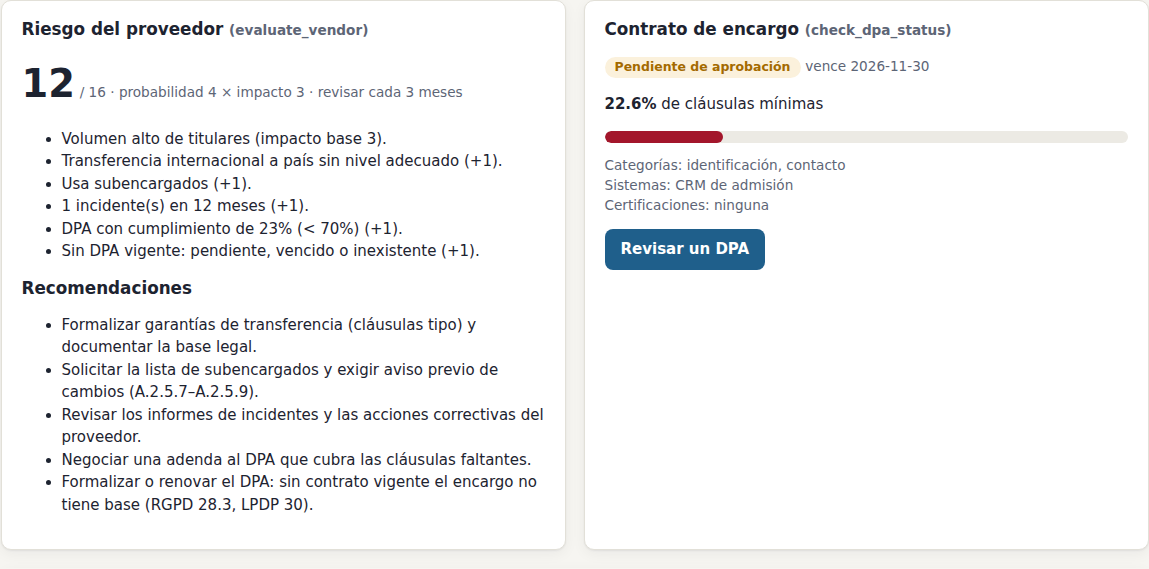
\includegraphics[width=\columnwidth]{../figuras/riesgo.png}\\[3pt]
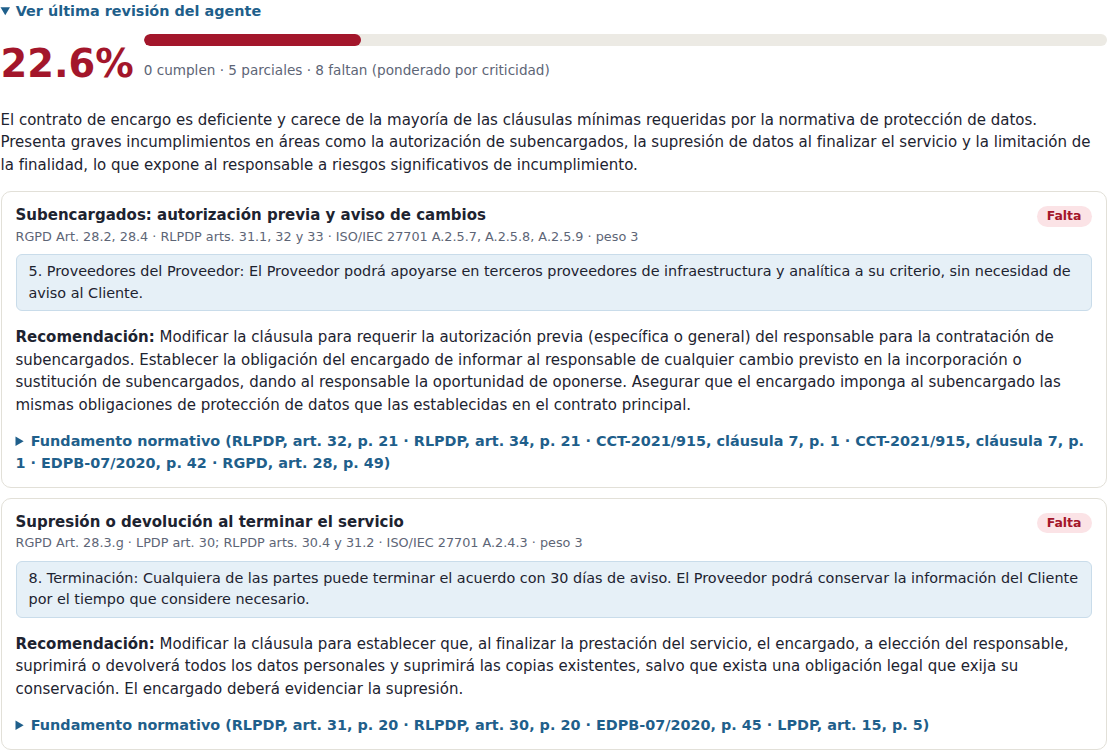
\includegraphics[width=\columnwidth]{../figuras/revision.png}
\caption{Interfaz del agente: riesgo del proveedor y estado del DPA (arriba); informe de revisión con citas y fundamentos (abajo).}
\label{fig:ui}
\end{figure}

%=====================================================================
\section{Discusión y limitaciones}
\begin{itemize}
  \item \textbf{Conjunto de evaluación pequeño.} Tres contratos anotados por los propios autores bastan para detectar errores gruesos, pero no para generalizar. El siguiente paso es anotar contratos reales anonimizados con un abogado.
  \item \textbf{Variabilidad del LLM.} Aun con temperatura 0{,}1, el estado de algunas cláusulas cambia entre corridas. La verificación literal y la aprobación humana mitigan el riesgo, pero no lo eliminan.
  \item \textbf{Etiquetado de artículos.} Un fragmento hereda el primer encabezado que contiene, así que el final de un artículo puede aparecer etiquetado con el siguiente. Esto afecta tanto a las citas como a la anotación de relevancia.
  \item \textbf{ISO/IEC 27701:2025.} No se indexa su texto y la numeración de los controles es inferida.
  \item \textbf{Documentos escaneados.} Los PDF que solo contienen imágenes requieren OCR, que todavía no está implementado.
\end{itemize}

%=====================================================================
\section{Conclusiones y trabajo futuro}
El Agente de Terceros automatiza la parte más repetitiva de la gestión de encargados: la lectura de contratos frente a las cláusulas exigibles. Además mantiene la trazabilidad normativa (fuente, artículo y página) y deja la decisión en manos humanas. Los \emph{embeddings} locales con FAISS mantienen la recuperación dentro de la organización. Al LLM externo solo se envían el contrato y los fragmentos públicos de la norma, nunca la base de datos personales, y una variante con un LLM local (Ollama) es directa. Como trabajo futuro planteamos: integrar el agente con el orquestador y con los agentes de Incidentes y de Controles a través del bus MCP; migrar el repositorio a la base PostgreSQL central del PIMS; generar adendas contractuales a partir de las cláusulas faltantes; y ampliar el conjunto de evaluación con contratos reales.

\bibliographystyle{IEEEtran}
\bibliography{referencias}

\end{document}
